\documentclass[a4paper,10pt] {article}
\usepackage[spanish]{babel}
\usepackage[utf8]{inputenc}
\usepackage{caratula}
\usepackage{a4wide}
\usepackage{graphicx}

\begin{document}

\titulo{Trabajo Pr\'actico Nro. 2}
\fecha{08/05/2009}
\materia{Algoritmos y Estructuras de Datos III}
\grupo{}
\integrante{Dinota, Mat\'ias}{076/07}{matiasgd@gmail.com}
\integrante{Huel, Federico Ariel}{329/07}{federico.huel@gmail.com}
\integrante{Leveroni, Luciano}{360/07}{lucianolev@gmail.com}
\integrante{Mosteiro, Agust\'in}{125/07}{agustinmosteiro@gmail.com}

\maketitle

\bigskip
\section*{Aclaraci\'ones generales}

Antes de comenzar el an\'alisis de cada ejercicio, cabe mencionar lo siguiente:

\begin{itemize}
 \item La implementaci\'on de los 3 algoritmos se realizó en \textbf{lenguaje Java}, haciendo uso de las librer\'ias est\'andar del mismo.
 \item Para el c\'alculo de tiempo de los algoritmos se utiliz\'o la funci\'on \textbf{nanoTime()} de la clase System de Java. Con el fin de aumentar la precisión de las mediciones, se utilizó el comando \textbf{nice} para darle máxima prioridad a la tarea.
 \item El c\'odigo fuente de los algoritmos aqui analizados se encuentran en los archivos \textit{Dengue.java} (Ej 1), \textit{...} (Ej 2) y \textit{...} (Ej 3).
 \item El c\'odigo fuente de los programas encargados de hacer uso de los algoritmos y necesarios para compilar las aplicaciones son:
 \begin{itemize}
    \item \underline{Ej 1:} MainDengue.java, Dengue.java e InstanciaDengue.java.
    \item \underline{Ej 2:} ...
    \item \underline{Ej 3:} ...
  \end{itemize}
 \item Para la lectura y escritura de los datos se utilizaron clases provistas por el lenguaje Java. No se har\'a referencia a estos algoritmos ya que no resultan de inter\'es para el trabajo aqui presentado.
 \item Al ejecutar cada programa sin argumentos se muestra una leyenda explicando su modo de uso.
 \item Los gr\'aficos se realizaron con \textbf{GNUPlot}. En los casos considerados pertinentes, se utiliz\'o una escala logar\'itmica con el fin de poder visualizar mejor los resultados.
\end{itemize}

\begin{center}
\section*{Ejercicio 1: Dengue}
\end{center}

\bigskip
\section*{Introducci\'on}

El objetivo del siguiente ejercicio es diseñar un algoritmo que resuelva el problema planteado de manera polinomial. Para esto se utiliz\'o la t\'ecnica de progamaci\'on din\'amica, lo que implic\'o la realizaci\'on de diversos pasos. Primero se corrobor\'o que el problema cumpla con el principio de optimalidad. Una vez comprobado esto (condici\'on necesaria para poder aplicar programaci\'on din\'amica) y utilizando las ideas vistas en dicha demostraci\'on, se procedi\'o a crear una funci\'on recursiva que retorne el resultado deseado. Luego se modific\'o dicha version por un algoritmo iterativo, siendo este un paso intermedio requerido para aplicar la t\'ecnica mencionada. El paso siguiente consisti\'o en modificar el algoritmo de manera de evitar la repetici\'on de c\'alculos innecesarios (aqu\'i queda implicita la idea de programaci\'on din\'amica), mejorando notablemente la complejidad de la funci\'on. Por \'ultimo, como veremos m\'as adelante, se opt\'o por un cambio de t\'ecnica algoritmica pasando de un algoritmo que originalmente era \textit{top-down} a uno \textit{bottom-up}.

\section*{Algoritmo}

En la presente sección presentaremos todos los pasos que se siguieron para lograr la implementación del algoritmo que resuelve el problema. Como se mencionó anteriormente, el problema será resuelto por medio de la técnica de programación dinámica por lo que presentaremos las demostraciones de todos los pasos que implica construir un algoritmo de esa manera. En primer lugar, se demostrará cómo aplica el principio de optimalidad en el problema dado. En segundo lugar, plantearemos una función recursiva que resuelva el problema y demostraremos su correctitud. Finalmente, mostraremos el algoritmo construido con programación dinámica, explicando detalladamente por qué resuelve el problema de manera más eficiente que la solución recursiva.

\subsection*{Principio de optimalidad}

Demostraremos por qu\'e vale el principio de optimilidad en este problema por el absurdo.

Sean $n$ y $l$ la cantidad de zonas y litros disponibles respectivamente y que las zonas se numeran de $1$ a $n$. Suponemos que la cantidad de mosquitos muertos con $l$ litros hasta la zona $n$ es \'optima y llamaremos $P$ a dicha cantidad. Sea $k$ la cantidad de litros usados en la zona $n$, suponemos que hasta la zona $n-1$ usando $l-k$ litros la cantidad de mosquitos muertos ($Q$) no es \'optima y se intenta llegar a un absurdo.

Si hasta la zona $n-1$ la cantidad de mosquitos muertos no es \'optima (para $l-k$ litros), existe otra forma de distribuir los $l-k$ litros entre las zonas $1$ a $n-1$ que hace que la nueva cantidad, a la que llamaremos $R$, sea \'optima (es decir, $R > Q$). Entonces tenemos que

$R + cantMM(n,k) > Q + cantMM(n,k) = P \Rightarrow R + cantMM(n,k) > P$

Esto es un absurdo ya que supusimos que $P$ era la cantidad \'optima. Este absurdo surge de suponer que la cantidad de mosquitos muertos hasta la zona $n-1$ con $l-k$ litros no era \'optima. Entonces queda demostrado que vale el principio de optimalidad para el problema planteado.

\subsection*{Solución recursiva y demostración de correctitud} %TODO!!!!!!!!!!!!!!!!!!!!!

A partir de la idea presentada en la secci\'on anterior se puede plantear la siguiente funci\'on recursiva para resolver el problema.
$\\ f(0, l) = 0 \\$
$ f(i,l) = max \left\{ \begin{array}{ll}
         f(i-1,l) & \mbox{$$}\\
        f(i-1, l-k) + MM[i][k] & \mbox{con $1 \leq k \leq l$}\end{array} \right. $


Siendo $MM[i][j]$ la matriz que contiene la cantidad de mosquitos muertos por litro, de cada zona. La soluci\'on al problema ser\'ia $f(n,l)$ con $n$ la cantidad de zonas y $l$ la cantidad de litros disponibles.

Para demostrar que la funci\'on presentada es correcta utilizaremos inducci\'on en la cantidad de zonas manteniendo la cantidad $l$ de litros fija. Es decir, queremos probar la siguiente proposición. \\

P(n): $f(n, i)$ es la cantidad máxima de mosquitos muertos hasta la zona $n$ con $i$ litros. ($0 \leq i \leq l$) \\

\textbf{Caso Base ($P(1)$)}

$f(1,i) = max_{1 \leq j \leq i} (MM[1][j]) \;\;\;\; $ con $i \leq 1$

Entonces, como se puede notar, $f(1,i)$ es trivialmente la cantidad máxima de mosquitos muertos de la primera zona con $i$ litros. \\

\textbf{Paso inductivo ($P(n) \Rightarrow P(n+1)$)}

Supongo que $f(n,i)$ es la máxima cantidad de mosquitos muertos hasta la zona $n$ con $i$ litros ($0 \leq i \leq l$) y demuestro que $f(n+1,i)$ es la cantidad máxima hasta la zona $n+1$.
Como $n+1 > 1$ tenemos que \\

$f(n+1,i) = max_{0 \leq k \leq i} (f(n, i-k) + MM[n+1][k])$ \\

Como $i - k \leq l$ para cualquier $k \leq i$ puedo aplicar la hipótesis inductiva, es decir, $f(n,i-k)$ es la máxima cantidad hasta la zona $n$ con $i-k$ litros. Entonces con $max_{0 \leq k \leq i} (f(n, i-k) + MM[n+1][k])$ obtengo la máxima cantidad de mosquitos muertos hasta la zona $n+1$ con $i$ litros pues $f(n,i-k)$ es máxima y se calcula el máximo para todas las cantidades $k$ de litros posibles para dicha zona. Entonces, como vale $P(1)$ y $P(n) \Rightarrow P(n+1)$ por principio de inducci\'on queda demostrada la proposici\'on.

La función presentada, a pesar de ser correcta, hace repetidas llamadas recursivas a valores ya calculados. Sin embargo, sirve de base para idear un algoritmo que use la técnica de programación dinámica para resolver este problema de forma más eficiente. En las posteriores secciones veremos en detalle cómo se relaciona dicha función con el algoritmo implementado.

\subsection*{Algoritmo utilizando programación dinámica}

A continuaci\'on se encuentra el pseudoc\'odigo del algoritmo que utiliza la técnica de programación dinámica para resolver el problema.

\begin{verbatim}
maxMMParcial[zonas][litros]

lleno la primer fila de maxMMParcial con 0

para i desde 1 hasta zonas
  para j desde 0 hasta litros
    max_parcial = maxMMParcial[i-1,j]
    k = 1
    mientras k <= j
      max_parcial = maximo(max_parcial, maxMMParcial[i-1,j-k] + MM[i][k])
    maxMMParcial[i][j] = max_parcial

guardar en Tp2Ej1.out la linea "maxMMParcial[zonas][litros]"


\end{verbatim}

% litrosPorZona[zonas]
% 
% litrosRestantes = litros
% j = litrosRestantes
% para i desde zonas hasta 1
%   mientras j >= 0 y (maxMMParcial[i][litrosRestantes] - MM[i-1][litrosRestantes - j]) != maxMMParcial[i-1][j]
%     j = j - 1
%   litrosPorZona[i-1] = litrosRestantes - j
%   litrosRestantes = j

% guardar en Tp2Ej1.out litrosPorZona

Este algoritmo está basado en la función recursiva presentada en la sección anterior, pero usando una estrategia \textit{Bottom-up} para calcular el resultado. Dicha estrategia se basa en el uso de una matriz para almacenar los resultados ya calculados y, a partir de ellos, construir las distintas etapas de la solución. Esta matriz tiene la siguiente forma:

\begin{center}
litros
\end{center}
\[ zonas \left( \begin{array}{ccccc}
0 & 0 & 0 & \cdots & 0 \\
0 & f(1,1) & f(1,2) & \cdots & f(1,l)  \\
0 & f(2,1) & f(2,2) & \cdots & f(2,l)	\\
\vdots & \vdots & \vdots & \ddots & \vdots \\
0 & f(n,1) & f(n,2) & \cdots & f(n,l) \end{array} \right)\]

En el algoritmo presentado cada fila de esta matriz se construye a partir de la fila anterior, por lo que la primer fila (que representa el caso base de $f$) debe ser 0 al comienzo del procedimiento. Además, en este cálculo también es necesario utilizar los valores de la matriz de entrada (MM) que contiene la cantidad de mosquitos muertos según la cantidad de zonas y litros.
Esto se corresponde a la definición recursiva de la función $f$ ya que el valor que retorna $f$ para cada zona $i$ se construye a partir de la zona $i-1$. 

Como se puede apreciar en el pseudocódigo cada elemento de la matriz se construye de la siguiente manera:

$ maxMMParcial[i][j] = max \left\{ \begin{array}{ll}
         maxMMParcial[i-1][j] & \mbox{$$}\\
        maxMMParcial[i-1][j-k] + MM[i][k] & \mbox{con $1 \leq k \leq j$}\end{array} \right. $


Esta definición muestra claramente la relación que existe entre el algoritmo que utiliza programación dinámica y la función que resuelve el problema de manera recursiva. Cada posición de la matriz se calcula de la misma manera que $f$, por lo que, si el caso base es el mismo, se obtendrán los mismos resultados. Por esta razón, al terminar de calcular toda la matriz (hasta la posición $n$ y $l$) se obtiene $f(n,l)$, es decir, la solución para la instancia del problema.


\section*{Complejidad}

En la presente secci\'on se calcular\'a la complejidad en el peor caso del algoritmo \textit{fumigar} bas\'andose en el modelo de c\'omputo uniforme. Esto se debe a que este ejercicio no se basa en el tama\~{n}o de los elementos de la matriz recibida como par\'ametro, sino en las dimensiones de dicha matriz, por lo que no se trabajar\'a con valores muy altos. Para realizar los c\'alculos de manera m\'as clara, se dividir\'a el analisis en el estudio de las dos partes que conforman la funci\'on: \textit{fumigaci\'on} y \textit{c\'alculo de litros por zona}

En la funci\'on \textit{fumigaci\'on} todas las operaciones y asignaciones utilizadas se logran en tiempo constante. Esto se debe al mencionado modelo de c\'omputo utilizado, en donde las operaciones presentes en el algoritmo no dependen del tama\~{n}o de los par\'ametros de entrada. De esta manera, la complejidad de esta funci\'on estar\'a supeditada al comportamiento de los ciclos que contiene. Llamaremos $a$ $b$ y $c$ a los ciclos, donde $a$ contiene a $b$ y este \'ultimo contiene a $c$. Se puede apreciar claramente que b itera $m$ veces (donde $m$ es la cantidad de litros) y que en cada iteraci\'on de b, se realiza una vez el ciclo c. El l\'imite de este ciclo esta dado por la variable de iteraci\'on de b (en el pseudoc\'odigo se llamada $j$), de manera que, en cada iteraci\'on de b, la cantidad de vueltas del ciclo c aumenta en uno, comenzando desde cero (valor de inicio de la variable $j$) hasta $m$. La complejidad del ciclo b sera entonces:

$$\sum_{j=0}^{m}j=\sum_{j=1}^{m}j=(m+1)m/2\ \in O(m^{2})  $$

El ciclo analizado se encuentra dentro de $a$, este \'ultimo se recorre $n$ veces (donde $n$ es la cantidad de zonas) debido a que su variable de iteraci\'on (en el pseudoc\'odigo llamada $i$) es inicializada en cero y aumentada en uno hasta llegar al valor $n$. Finalmente podemos concluir que la complejidad de la funci\'on \textit{fumigaci\'on} es:

$$T(n,m)=n((m+1)m/2)\ \in O(nm^{2})$$


Por otro lado, analizaremos la complejidad en peor caso de la otra parte del algoritmo: \textit{c\'alculo de litros por zona}. En cuanto a los costos de las operaciones matem\'aticas y asignaciones, sucede lo mismo que en el caso anterior por lo que nuevamente el estudio de la complejidad se concentrar\'a en los ciclos. En este caso tenemos dos ciclos. Se puede apreciar facilmente que el ciclo externo realiza $n$ iteraciones ya que la variable $i$ utilizada para iterar es inicializada en $n$ y es decrementada hasta llegar a 1. Como muestra el pseudoc\'odigo, el limite del ciclo interno esta dado por una condici\'on por lo que la cantidad de iteraciones que realize var\'ia cada vez que es ejecutado. Lo que si se puede ver es que, en total (es decir, para las $n$ iteraciones del ciclo externo), el ciclo ser\'a recorrido $m$ veces. Esto se debe a que en caso de cumplir con la condici\'on mencionada, la variable de iteraci\'on del ciclo $j$ es decrementada en 1, y nunca es reiniciada. Como dicha variable es inicializada con la cantidad de litros y en cada vuelta del ciclo interno se corrobora que su valor sea mayor o igual que cero, podemos concluir que dicho ciclo ser\'a recorrido $m$ veces en total (ya que si se cumple la condici\'on, $j$ es decrementado, y si no se satisface la guarda, no se entra al ciclo). Por estos motivos la segunda parte del algoritmo de \textit{fumigar} tiene complejidad $T(n)\ \in O(n+m)$.


De esta manera, como la complejidad de la primer parte de la funci\'on pertenece a $O(nm^{2})$, la segunda pertenece a $O(n+m)$ y $O(n+m)\ \in O(nm^{2})$, concluimos que la complejidad en peor caso del algoritmo \textit{fumigar} es $$T(n,m) \in O(nm^{2})$$


Finalmente estudiaremos la complejidad en funci\'on del tama\~{n}o de la entrada. Sea $t$ el tama\~{n}o de la entrada, $n$, $m$ y $M$ la cantidad de zonas, litros y la matriz pasados como par\'ametros respectivamente. Tenemos entonces que:

$$t=\log(n)+\log(m)+\sum_{i=1}^{n}\sum_{j=1}^{m}\log(M_{i,j})>\log(n)+\log(m)+\sum_{i=1}^{n}\sum_{j=1}^{m}1>\log(n)+\log(m)+nm>nm$$


\hspace{45pt} $\Longrightarrow$ como $T(n,m) \in O(nm^{2})$ y $nm^{2}<(nm)^{2}<t^{2} \Longrightarrow T(t) \in O(t^{2})$


\section*{An\'alisis de resultados}

Con el fin de analizar la complejidad de los algoritmos propuestos (fumigación y cálculo de litros por zona) se realizaron varias pruebas. Estos experimentos están orientados a estudiar el tiempo de ejecución del mismo en relaci\'on a los datos de entrada, comparando el costo real de los algoritmos junto con su complejidad teórica calculada. Para cada algoritmo se verán 3 gráficos distintos. El primero de ellos servirá para analizar la complejidad con respecto a los litros, es decir, fijando la cantidad de zonas. Reciprocamente, el segundo será en base a la cantidad de zonas con una cantidad fija de litros. Por último, el tercer gráfico en 3 dimensiones mostrará como se comporta el algoritmo considerando ambas variables en conjunto.

A continuación se describirán las características de las instancias utilizadas para las pruebas así como las particularidades de cada experimento. Dichas cuestiones son comunes al analisis de ambos algoritmos por lo que no haremos referencia a ninguno en particular. Más adelante analizaremos resultados de estos experimentos aplicado a cada uno de los algoritmos.

Para las instancias de prueba se utilizó la función \textit{random} del lenguaje para generar matrices de \textit{mosquitosMuertos}) de tamaño $zonas*litros$ con valores aleatorios comprendidos entre $1$ y $10000$ con el fin de garantizar que las pruebas resulten lo suficientemente genéricas como para poder obtener resultados ``interesantes''. Cabe mencionar que no se harán estudios sobre instancias particulares ya que, como se mencionó antes, el costo de ejecución del algoritmo de \textit{fumigación} no depende de los valores de la matriz de entrada que conforma cada instancia.

En primer lugar, se hicieron cálculos utilizando como variable la cantidad de zonas a fumigar, fijando en $10$ los litros disponibles. El rango de zonas analizados es desde $1$ hasta $10000$ zonas, de a intervalos de tamaño $10$. La elección de estos valores fue producto del análisis de 2 cuestiones importantes: que números permitirían tomar muestras utiles para la realización de los gráficos y cual era la máxima cantidad de datos que nuestra aplicación podría manejar, acotada por el tiempo disponible para realizar las pruebas y las limitacion propias de la máquina en cuestión. Empiricamente, se comprobó que dicho rango de zonas permitía correr la aplicación en un tiempo razonable y al mismo tiempo proveer datos interesantes para el análisis en cuestión. Del mismo modo, fijar en 10 los litros aseguró que sea la cantidad de zonas el parámetro ponderante en el cálculo de tiempo de ejecución.

La segunda prueba resulta muy similar a la anterior en cuanto al rango de valores utilizados. La diferencia radica en que ahora el parámetro fijado es la cantidad de zonas en vez de la cantidad de litros, variando los litros en el rango $1$ hasta $10000$, de a intervalos de tamaño $10$ (al igual que en la prueba anterior).

La tercer y última prueba consistió en analizar el algoritmo considerando ambas variables en conjunto, de modo de poder comparar el tiempo de ejecución para distintos valores de zonas y litros junto con la complejidad teórica que depende de estos dos parámetros. Para esta prueba se tomaron valores de zonas y litros entre $1$ y $1000$, de a intervalos de tamaño $100$ (10 valores posibles). Luego, se calcularon los tiempos de ejecución de todas las permutaciones de los 10 elementos pertenecientes a dicho conjunto de manera tal de obtener resultados para las combinaciones de litros y zonas dentro del intervalo mencionado.

A continuación se presentarán los gráficos realizados para cada algoritmo utilizando estas 3 pruebas descriptas.

\subsection*{Fumigación}

Como se vió anteriormente, la primer parte del problema consistía en calcular la máxima cantidad de mosquitos muertos para una instancia determinada. Los siguientes gráficos muestran el comportamiento de este algoritmo en base a los dos parámetros de entrada de manera independiente:

\begin{center}
 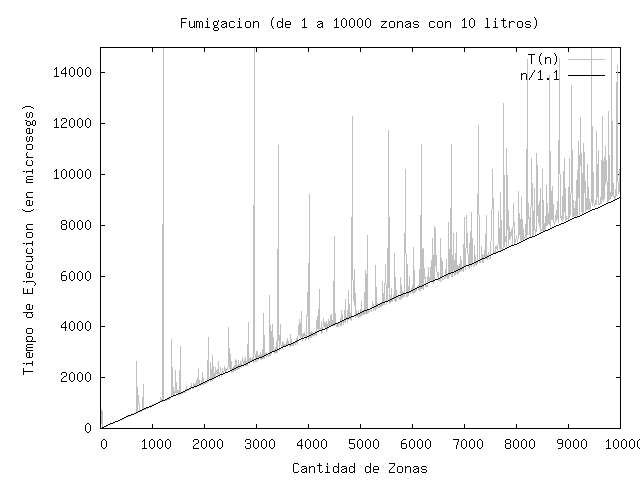
\includegraphics[width=0.7\textwidth]{Plots/Tp2Ej1-TiemposFumigacionPorZonas-10litros-bw.png}
\begin{center}
Figura 1.1
\end{center}
 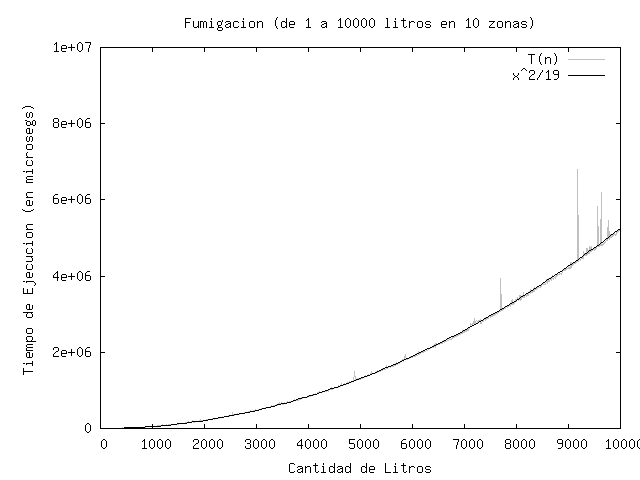
\includegraphics[width=0.7\textwidth]{Plots/Tp2Ej1-TiemposFumigacionPorLitros-10zonas-bw.png}
\begin{center}
Figura 1.2
\end{center}
\end{center}

Ambos gráficos permiten observar algunas cuestiones interesantes. La Figura 1.1 permite observar como el comportamiento del algoritmo de \textit{fumigación} con respecto a la cantidad de zonas se asimila a una función lineal, hecho que se corresponde con la complejidad calculada anteriormente. Del mismo modo, la Figura 1.2 muestra como la función T(n) que representa el tiempo de ejecución se comporta prácticamente igual que la función $f(n) = n^2/19 \in O(n^2)$. Este hecho demuestra empíricamente que la complejidad con respecto a la cantidad de litros es cuadrática al realizar la fumigación tal como se había analizado anteriormente.

Otras cuestión observable son los ``picos'' y variaciones abrutas en ambos gráficos. En principio, esto no debería ocurrir ya que la complejidad no depende de la forma de la entrada como se mencionó anteriormente. El motivo de esto radica simplemente en los errores de precisión en la medición de las operaciones propios de las limitaciones de la máquina de cómputo utilizada. Los tiempos de ejecución del algoritmo son mucho mayores en la Figura 1.2 lo que resulta en una mayor estabilidad en los cálculo de tiempo, en contraste con la Figura 1.1 donde hay mayor impresición porque dicho gráfico refleja cambios de valores más abrutos.

\begin{center}
 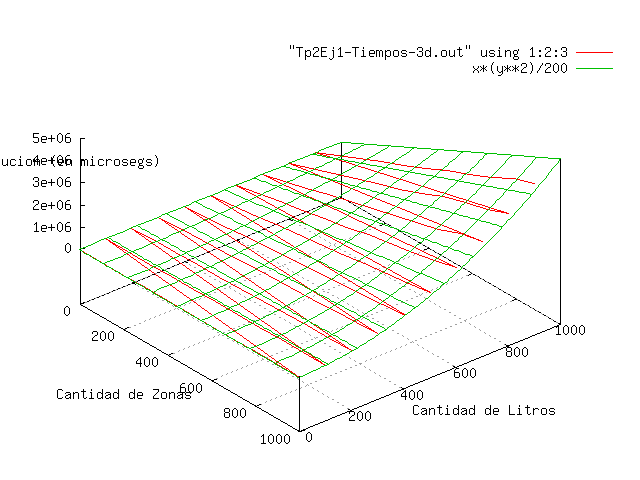
\includegraphics[width=0.7\textwidth]{Plots/Tp2Ej1-TiemposFumigacion-3d-bw.png}
\begin{center}
Figura 1.3
\end{center}
\end{center}

Esta última figura permite ver como el algoritmo en su totalidad realmente se comporta de la forma esperada. 
Para esto basta comparar los tiempos de ejecución al variar ambos parámetros (litros y zonas) junto con la función $f(n,m) = n*m^2/200 \in O(n*m^2)$ viendo que ambas ``mantas'' coiniciden. Este ultimo hecho constituye la última prueba de que empirícamente el algoritmo funciona tal como se esperaba.

\subsection*{Cálculo de Litros Por Zona}

En esta sección analizaremos el comportamiento del otro algortimo propuesto que se encarga de dar parte de la solución del problema: el algoritmo encargado de calcular los litros a utilizar por cada zona. Los siguientes gráficos muestran el comportamiento del mismo en base a las dos variables en cuestión de forma independiente:

\begin{center}
 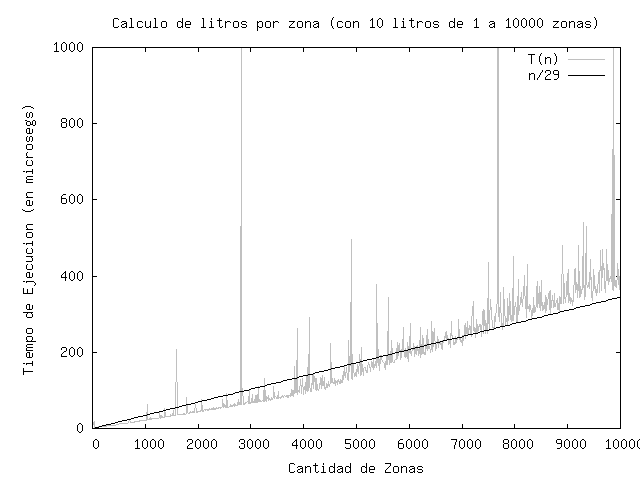
\includegraphics[width=0.7\textwidth]{Plots/Tp2Ej1-TiemposLitrosPorZonaPorZonas-10litros-bw.png}
\begin{center}
Figura 2.1
\end{center}
 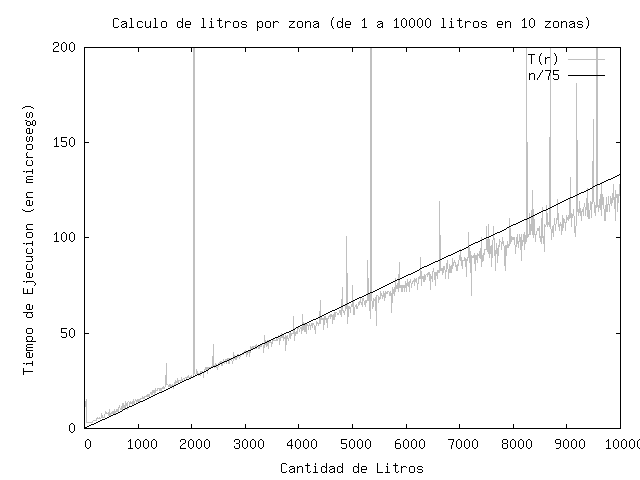
\includegraphics[width=0.7\textwidth]{Plots/Tp2Ej1-TiemposLitrosPorZonaPorZonas-10zonas-bw.png}
\begin{center}
Figura 2.2
\end{center}
\end{center}

Como se puede observar, en ambos casos, el comportamiento del algoritmo es el esperado. La Figura 2.1 muestra como el cálculo de litros por zona se ``corresponde'' con el gráfico de la función lineal $f(n) = n/25$ al variar la cantidad de zonas y fijar los litros en $10$. Asímismo, la Figura 2.2 se comporta de la forma $f(n) = n/75$ al variar los litros y fijar las zonas. Esto comprueba la linealidad en complejidad teórica analizada previamente para ambas variables. Un punto interesante a observar es que las constantes que acompañan a estas funciones difieren, siendo la constante relacionada al primer gráfico ($1/25$) 3 veces mayor que la otra ($1/75$). Al tratarse de instancias de igual tamaño (en ambos casos, matrices desde $1*10$ hasta $10000*10$), se puede concluir que la \textit{performance} de este algoritmo depende en mayor medida de la cantidad de zonas que de la cantidad de litros. En otras palabras, para instancias de igual tamaño, un caso demora 3 veces más el otro. \textbf{POR QUE?}

Con respecto a la irregularidad del gráfico, cabe notar que, a diferencia del algoritmo anterior, este algoritmo no realiza siempre la misma cantidad de operaciones para instancias de igual tamaño tal como se vió en la sección de análisis de complejidad, ya que el recorrido inverso de la matriz resultante depende justamente de los valores que esta contenga que dependen a su vez de los valores de la matriz de entrada \textit{mosquitosMuertos} (ver sección \textit{Algoritmo}). Por este motivo, debido a que se trata de instancias aleatorias, es esperable que no se obtenga un comportamiento ``tan'' similar a la función lineal propuesta como ocurre para el primer algoritmo.

Por último, al igual que para el algoritmo anterior, se presenta el siguiente gráfico de 3 dimensiones:

% \begin{center}
%  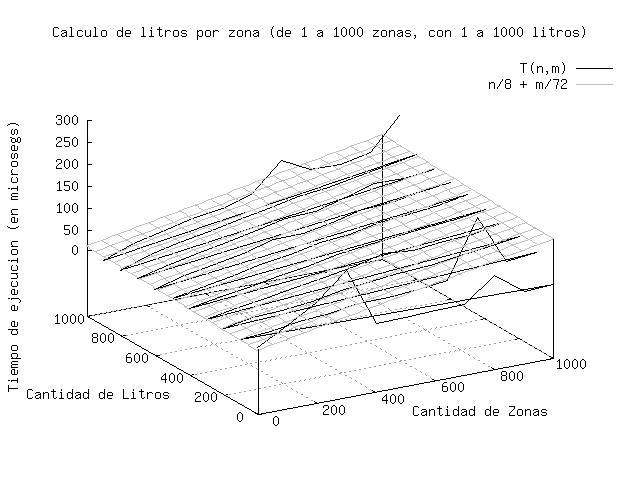
\includegraphics[width=0.7\textwidth]{Plots/Tp2Ej1-TiemposLitrosPorZona-3d-bw.png}
\begin{center}
Figura 1.3
\end{center}
% \end{center}

Al igual que antes, este gráfico permite ver la complejidad de ambos parámetros en conjunto. \textbf{TODO}

\section*{Conclusiones}

%TODO: Decir que se podria haber analizado los algoritmos recursivos que repiten operaciones vs la programacion dinamica pero no hubo tiempo.

% Este ejercicio nos mostr\'o un caso representativo en el que el tiempo de ejecuci\'on difiere notablemente a la complejidad calculada para el peor caso.
% 
% Para este algoritmo en particular se debe a que la funci\'on \textit{encontrarPrimos} alcanzar\'ia dicho peor caso si la conjetura de Goldbach fuese falsa, cuesti\'on que no sucede para ning\'un n\'umero que pueda tomar la func\'on (es decir, hasta el n\'umero mas grande almacenable en un \textit{int}). M\'as aun, esta demostrado que para n\'umeros mucho mas grandes que los testeados la conjetura se sigue cumpliendo (ver secci\'on Referencias para m\'as detalles) por lo que en el \'ambito cient\'ifico se cree que es cierta.
% 
% Tambi\'en vimos casos en los que entre n\'umeros cercanos tomados por la funci\'on, el tiempo de ejecuci\'on difiere considerablemente. Adem\'as notamos que a medida que el tama\~{n}o del par\'ametro de entrada crece el tiempo tamb\'ien lo hace, pero siempre muy lejos de los peores casos para dichas entradas. Estas situaciones se deben a la desconocida distribuci\'on de los n\'umeros primos entre los naturales, por lo que no podemos dar una explicaci\'on general que incluya todos los casos reales. Sin embargo, en base a todos los an\'alisis realizados, podemos concluir que para todos los casos computables por nuestro algoritmo el tiempo de ejecuci\'on ser\'a mas que aceptable.

TODO

\bigskip

\begin{center}
\section*{Ejercicio 2: Encontrar Diamante en un grafo}
\end{center}

\bigskip
\section*{Introducci\'on}

El objetivo del siguiente ejercicio es dise\~{n}ar un algoritmo que, dado un grafo, encuentre el menor subgrafo inducido isomorfo a un diamante, en caso de que éste exista. Un diamante puede definirse como un grafo $K_{4}$ menos una arista. Este algoritmo está basado en una propiedad sobre diamantes (enunciada en el Anexo A) que, además de ser usada para resolver el problema, será demostrada de manera formal.

En un principio, cuando se comenzó a idear el algoritmo, surgió la idea de utilizar solamente la propiedad enunciada para resolver el problema. Es decir, para toda vecindad de cada nodo, estudiar cada componente conexa para determinar si la misma es completa. Sin embargo, esto sólo aportaba información sobre las componentes conexas que formaban un diamante, pero no brindaba detalles sobre los nodos que formaban el diamante, y no aseguraba que este fuera mínimo para dicha componente conexa. Por esta razón, se optó por utilizar un método más complejo que, aunque se basa en la propiedad mencionada, obtiene de cada componente conexa no completa (existe diamante) los nodos mínimos que forman un diamante. Esto se realiza calculando el mínimo nodo que puede formar un diamante y, a partir de este, construir el mínimo probando las posibles combinaciones que construyan un diamante. De esta manera se pueden obtener los diamantes mínimos de cada componente conexa no completa de una determinada vecindad y así determinar el mínimo de la misma. Finalmente, se comparan los diamantes obtenidos de cada vecindad para obtener el mínimo diamante del grafo. Este algoritmo será explicado en detalle, se mostrará su correctitud y se presentará la implementación y pruebas de ejecución del mismo en posteriores secciones.

\section*{Algoritmo}

A continuaci\'on se presenta el pseudoc\'odigo del algoritmo para resolver el problema propuesto.

\begin{verbatim}
leer archivo y crear adyacencias excepto para los nodos de grado 1 y 0, un arreglo donde cada posicion i es una lista de los nodos adyacentes del nodo i

Armar la matriz de adyacencias

para cada nodo (que llamaremos superNodo) del grafo
  si el tamaño de la lista de adyacencia de superNodo es mayor que 3
    vecindadDeSuperNodo = crearVecindad(superNodo)
    agregar buscarDiamanteMinimoEnVecindad(vecindadDeSuperNodo) a diamantesMinimos

diamanteMinimo = minimo(diamantesMinimos)
guardar en "Tp2Ej2.out" diamanteMinimo


crearVecindad(superNodo) //O(m)
  para cada nodo k de adyacencias[superNodo]
    para cada nodo j de adyacencias[k]
      si nodo j es adyacente a superNodo
        agregar nodo j a listaVecindad
    vecindadDeSuperNodo[k] = listaVecindad
  devolver vecindadDeSuperNodo //esto es un grafo (array de listas de adyacencia)

\end{verbatim}

Antes de comenzar, para la implementaci\'on se utilizaron las siguientes estructuras:
\begin{itemize}
 \item \textbf{tablero:} es la matriz en donde se ir\'an colocando las fichas que son posible soluci\'on hasta un paso determinado. Fue implementada mediante un arreglo de arreglos.
\item \textbf{fichas:} es el arreglo que contiene todas las fichas de entrada del algoritmo (provenientes de Tp1Ej2.in).
\item \textbf{fichaActualEn:} cada posici\'on de esta matriz contiene la posici\'on en el arreglo fichas de la ficha actual (la ficha que est\'a siendo evaluada como soluci\'on del tablero en un paso del algoritmo) para cada una de las casillas del tablero. Al igual que tablero, esta estructura est\'a implementada con un arreglo de arreglos.
\item \textbf{fichasPuestas:} es un arreglo de datos \textit{booleanos} del mismo tama\~{n}o que fichas, que indica si una determinada ficha est\'a colocada en el tablero.
\item \textbf{jardineroViejo/Nuevo:} estructura implementada a trav\'es de una lista enlazada, que se utiliza, como veremos m\'as adelante, para aplicar las podas del algoritmo.
\end{itemize}

Luego de inicializar las estructuras, comienza el ciclo principal que intentar\'a colocar las fichas de una en una en el tablero finalizando una vez que este se complete (es decir, cuando $i = n$). En primer lugar se verifica que la ficha actual, apuntada por fichaActualEn[i][j], encaje en la posici\'on (i,j) del tablero y que la misma no pertenezca al conjunto de fichas puestas. En caso afirmativo, se procede a evaluar si se puede realizar una poda (posteriormente explicada en la secci\'on Poda). De no ser factible esta \'ultima, se coloca la ficha en el tablero y se avanza a la siguiente posici\'on del mismo. Si se llega a aplicar la poda, la ficha no se inserta.

En caso de que no se haya insertado una ficha en alg\'un paso del algoritmo, se intentar\'a colocar la siguiente ficha (es decir, se aumenta fichaActualEn[i][j]). Si la ficha revisada resulta ser la \'ultima por revisar, se retrocede hasta la posici\'on del tablero m\'as cercana que tenga fichas por revisar a\'un. Como se sugiri\'o anteriormente, dicha comprobaci\'on se realiza por medio de la matriz fichaActualEn. Si se intentara retroceder de la posici\'on inicial (0,0) la instancia recibida no tiene soluci\'on y, por lo tanto, el algoritmo finaliza informando tal evento.

\subsection*{Poda}

Con el fin de optimizar el rendimiento del algoritmo se aplicó el concepto de \textit{poda} visto en clase, relativo a todo algoritmo de \textit{backtracking}. La poda propuesta consiste en la siguiente idea que veremos a continuaci\'on. Cabe aclarar que esta poda no se aplica a los bordes izquierdo e inferior del tablero, ya que idea en cuesti\'on no es aplicable en dichas posici\'ones.

En primer lugar, cada vez que se desea añadir una ficha, se genera un conjunto determinado de fichas relacionadas a la misma que llamaremos ``jardinero''. Un ``jardinero`` est\'a conformado por todas las fichas que pueden unirse por debajo con la ficha a la cual est\'a asociada el jardinero. . Como se puede ver en el pseudoc\'odigo, una vez que se verific\'o que la ficha actual es candidata para ser insertada en el tablero (aquella que encaja en la posici\'on actual seg\'un lo visto antes) se crea el jardinero asociado a esa ficha que denominaremos \textit{jardineroNuevo}. En el caso de encontrarse en el borde izquierdo del tablero, la poda no se aplica y simplemente \textit{jardineroNuevo} pasa a ser \textit{jardineroViejo}. Este \'ultimo siempre va a ser el jardinero asociado a la ficha anterior a la posici\'on actual del tablero. 

Para los casos no pertenecientes al borde izquierdo (ni inferior), se evalua si se puede realizar la poda mediante la func\'ion \textit{puedoPodar(jardineroViejo, jardineroNuevo)}. Tal como muestra el pseudoc\'odigo, la misma verifica si hay intersecci\'on entre ambos jardineros, es decir, si alguna de las fichas de un jardinero puede encajar con alguna ficha del otro. Si ninguna encaja, implica que la ficha actual (\textit{fichas[fichaActualEn[i][j]]}) que se estaba por insertar no puede ir junto con la ficha anterior (ficha a su izquierda) en esa ubicaci\'on del tablero (quiz\'as si pueden formar parte del borde inferior). Observando este hecho desde el punto de vista de un algoritmo de \textit{backtracking}, al descartar esta posible soluci\'on se evita tener que ver todas las soluciones que involucren el haber insertado tal ficha en el tablero, evitando as\'i tener que analizar esa ''rama`` del \'arbol k-ario de posibles soluciones. Por este motivo, podemos afirmar que este procedimiento realizado constituye una \textit{poda} del \'arbol de \textit{backtracking}.

Para poder mantener el invariante de tener siempre un jardinero asociado a la ficha anterior a la actual (\textit{jardineroViejo}) es necesario contemplar el caso en el que se retrocede a posiciones anteriores del tablero y se retira fichas insertadas anteriormente. En tal caso, como se puede ver en el pseudoc\'odigo, se genera un \textit{jardineroViejo} que se asocia la posici\'on anterior a la actual (es decir, la posici\'on (i\_ant, j\_ant)). De este modo, al iterar nuevamente, el jardinero de la nueva ficha a insertar (jardineroNuevo) puede evaluarse con el jardineroViejo para ver si se puede realizar una nueva poda.

Como veremos enseguida, esta poda resulta efectiva en la pr\'actica, disminuyendo notoriamente los tiempos de ejecuci\'on.

\section*{Complejidad}

Como el algoritmo propuesto se basa en la t\'ecnica de \textit{backtracking}, la complejidad del mismo en el peor caso es similar a la de un algoritmo de fuerza bruta. En este tipo de algoritmos, se generan todas las soluciones posibles y se eval\'uan para determinar si cumplen con el problema a resolver. La complejidad de generar y revisar todas las soluciones posibles es exponencial y, en particular, el algoritmo de fuerza bruta aplicado al problema presentado ser\'ia $O(n!)$, con $n$ la cantidad de fichas del tablero. A pesar de que los algoritmos de \textit{backtracking} descartan gran cantidad de casos y aplican podas para reducir el tiempo de ejecuci\'on, existen casos patol\'ogicos en que pocas de estas optimizaciones pueden ser utilizadas y, por lo tanto, se recorran todas las ramas de soluciones. Estos casos hacen que la complejidad en el peor caso del algoritmo presentado sea la misma que la de un algoritmo de fuerza bruta, es decir $O(n!)$ (siendo $n$ la cantidad de fichas totales del tablero). Sin embargo, como estudiaremos en posteriores secciones, el tiempo de ejecuci\'on del algoritmo difiere significativamente del tiempo del algoritmo de fuerza bruta.

\section*{An\'alisis de resultados}

En la siguiente secci\'on se mostrar\'an los an\'alisis realizados para tableros de distinto tama\~{n}o. El enfoque principal de las pruebas radica en estudiar los tiempos de ejecuci\'on del algoritmo con y sin la poda. Para esto se implement\'o un algoritmo que genera tableros aleatorios de un tama\~{n}o $n$ pasado como par\'ametro. De esta manera, utilizando dicho algoritmo para distintos valores de $n$, se contrastaron ambos metodos (con y sin poda) con la cota estudiada ($n!$) arrojando los siguientes resultados. Vale aclarar que se utiliz\'o una escala logar\'itmica sobre el eje de ordenadas ya que los tiempos de ejecuci\'on toman valores muy altos, adem\'as, para realizar los gr\'aficos expuestos, se utilizaron tableros hasta un tama\~{n}o de $n=15$ pues para mayores valores los tiempos son excesivos.

% \begin{center}
%  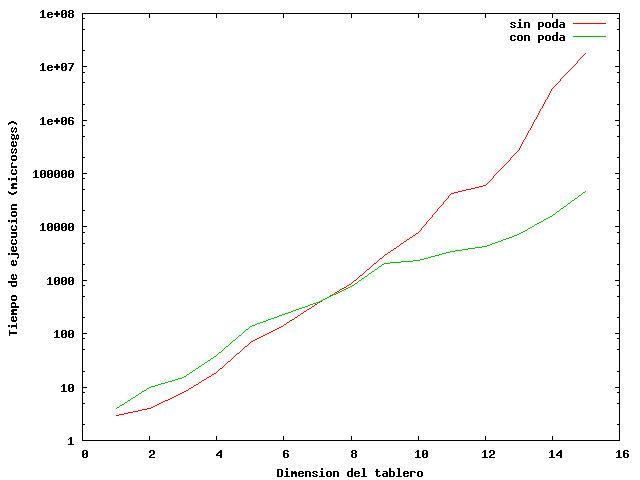
\includegraphics[width=0.7\textwidth]{Plots/Ej2-Complejidad2.png}
% \begin{center}
% Figura 2.1
% \end{center}
% \end{center}
% 
% \begin{center}
%  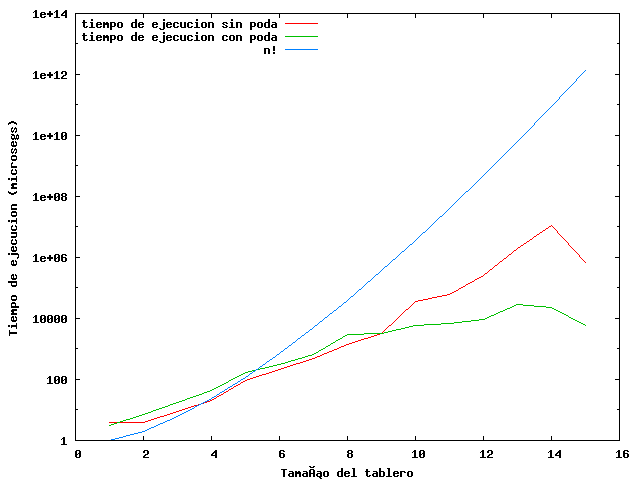
\includegraphics[width=0.7\textwidth]{Plots/Ej2-Complejidad1.png}
% \begin{center}
% Figura 2.2
% \end{center}
% \end{center}

Como se puede apreciar en ambos gr\'aficos, los tiempos de ejecuci\'on de los dos algoritmos son sensiblemente menores que los de la complejidad teorica calculada para el peor caso ($O(n!)$). Esto concuerda con lo esperado ya que como se dijo en anteriores secciones, salvo en casos patol\'ogicos, en la pr\'actica el metodo de \textit{backtracking} aplicado a este problema es mucho m\'as eficiente.

Con respecto a las diferentes resultados obtenidos con los dos m\'etodos, vemos reflejado que efectivamente la poda produce una importante mejora en el rendimiento. Si bien para tableros peque\~{n}os el rendimiento es similar (es m\'as, en la mayor\'ia de los casos para $n$ chicos el m\'etodo que utiliza la poda suele ser menos eficaz), esto no es de importancia ya que en dichos casos, al no manejar gran cantidad de datos, el tiempo de ejecuci\'on no alcanza valores muy altos. Por el contrario, cuando tomamos valores de $n$ mas grandes (aprox $n\geq10$), se puede apreciar que la poda descarta gran cantidad de soluciones no posibles, lo que incide directamente en la eficiencia de la aplicaci\'on. De hecho, cuando se analizaron tableros de tama\~{n}o mayor que 15, el tiempo que llev\'o a cabo el algoritmo sin la poda para buscar una soluci\'on result\'o excesivo, situaci\'on que no ocurre cuando se utiliza la poda para tableros de hasta $n=25$.

Por \'ultimo, cabe notar que el tiempo de ejecuci\'on real no est\'a estrictamente relacionado con el tama\~{n}o de entrada. Podemos apreciarlo en la \textit{Figura 2.2}, donde la ejecuci\'on de el algoritmo con y sin la poda tom\'o m\'as tiempo para $n=14$ que para $n=15$. Esto se debe a que, adem\'as de depender de la dimensi\'on del tablero, la eficiencia del algoritmo estar\'a relacionada con la distribuci\'on de las fichas recibidas.

\section*{Conclusiones}

A lo largo del desarrollo del ejercicio, se experimentaron las particularidades de un algoritmo de \textit{backtracking}. Nos encontramos con diversas dificultades en la implementaci\'on, a pesar de que la idea intuitiva del algoritmo es relativamente simple. Adem\'as, llegamos a la conclusi\'on de que, si bien la complejidad en peor caso es muy elevada, el algoritmo en general suele ser mucho m\'as eficiente que algoritmos que utilizan la t\'ecnica de fuerza bruta para resolver este tipo de problemas. 

Los principales incovenientes que surgen al implementar un algoritmo de \textit{backtracking} tienen que ver con la elecci\'on de la poda. Al momento de dicha elecci\'on, se deben considerar los aspectos de eficiencia, dificultad en la implementaci\'on y sobre todo, los beneficios (en relaci\'on al tiempo de ejecuci\'on) que esta provocar\'ia. Al pensar en detalle cada uno de las posibles podas, estos factores fueron determinantes para tomar una decisi\'on; podas que parec\'ian muy eficientes en principio, resultaban muy dif\'iciles de implementar y no aportaban cambios significativos que justifiquen su uso. A su vez, podas que parec\'ian descartar muchos casos, terminaban empeorando el tiempo de ejecuci\'on.

Es importante destacar que al aplicar la poda propuesta, el algoritmo mejora considerablemente en promedio. Esta situaci\'on resultaba esperable y pudo ser comprobada emp\'iricamente en las pruebas realizadas. Tambi\'en, se not\'o una relaci\'on entre la distribuci\'on de fichas de entrada y el tiempo de ejecuci\'on del algoritmo presentado. Por ejemplo, existen casos en los que la disposici\'on de las fichas no permitan hacer podas y otros en los que no sea necesario tener que reemplazar alguna ficha.

En conclusi\'on, la eficiencia del algoritmo de \textit{backtracking} depende fuertemente de las podas que se realicen y de la distribuci\'on probabil\'istica de los par\'ametros de entrada para casos promedio. Por esta raz\'on, la implementaci\'on de podas es determinante y justifica el tiempo invertido en idear las mismas.

\begin{center}
\section*{Ejercicio 3: C\'alculo de la mediana entre dos vectores}
\end{center}

\bigskip
\section*{Introducci\'on}

El problema que plantea este ejercicio es calcular la mediana entre dos vectores de n\'umeros enteros, es decir, el elemento que, una vez concatenados y ordenados los vectores, deja a ambos lados la misma cantidad de elementos. Seg\'un lo especificado en el problema, ambos vectores tienen la misma longitud y est\'an ordenados.

En principio, la soluci\'on trivial del problema fue descartada ya que el costo de realizarla era excesivo para los fines del ejercicio. Esta soluci\'on consist\'ia en concatenar ambos vectores, ordenarlos y posteriormente obtener la mediana a partir del elemento medio de dicha secuencia.

Descartada esta opci\'on, surgi\'o la idea de desechar una gran cantidad de elementos, cuando sea posible, para poder realizar los c\'alculos sobre una cantidad de n\'umeros considerablemente inferior a la inicial. De esta manera, la complejidad resultar\'ia del costo de descartar los elementos apropiados y luego hacer el c\'alculo con una cantidad peque\~{n}a de elementos. Evidentemente, nuestro algoritmo seguir\'ia el concepto de Divide and Conquer cl\'asico.

Con las ideas m\'as claras, notamos que descartando la misma cantidad de elementos mayores o iguales a la mediana, que menores o iguales a ella, \'esta se manten\'ia como valor medio de los vectores generados a partir de los elementos no descartados. R\'apidamente, nos dimos cuenta que la mediana de concatenar dos vectores ordenados, se encuentra entre los elementos mayores a la mediana del vector con menor valor medio y los elementos menores a la mediana del vector con mayor valor medio (conjetura que luego se demostrar\'a).

Planteado todo esto, result\'o sencillo escribir el pseudoc\'odigo de nuestro algoritmo. 

\section*{Algoritmo}

A continuaci\'on se mostrar\'a el pseudoc\'odigo del algoritmo implementado seguido de una demostraci\'on de su correctitud.

\begin{verbatim}
medianaRecursiva (vector x[0..n-1], vector y[0..n-1])

  si n == 1
    si x[0] > y[0]
      devolver y[0]
    sino
      devolver x[0]

  si n == 2
    si x[0] == y[0]
      devolver x[0]
    si x[0] > y[0]
      si x[0] > y[1]
        devolver y[1]
      sino
        devolver x[0]
    sino
      si x[1] > y[0]
        devolver y[0]
      sino
        devolver x[1]

  si n > 2
    si n es impar
      medio = n / 2
    sino
      medio = n / 2 - 1;
    si x[medio] > y[n/2]
      devolver medianaRecursiva(x[0..medio], y[n/2..n-1]);
    sino
      devolver medianaRecursiva(x[medio..n-1], y[0..n/2]);
\end{verbatim}

Con respecto a la implementaci\'on del algoritmo, la misma result\'o bastante sencilla de realizar en el lenguaje C++, utilizando las operaciones b\'asicas que provee el lenguaje y usando arreglos b\'asicos para la reprentaci\'on de los vectores. La \'unica parte no trivial radica en el uso de punteros para lograr llamar recursivamente a la func\'on con las ``mitades'' correspondientes de cada arreglo. Tambi\'en, cabe notar que en la implementaci\'on fue necesario pasar como par\'ametro extra el tama\~{n}o de los arreglos que reprentan a los vectores por cuestiones intr\'insicas al manejo de arreglos din\'amicos en C++.

Como se puede apreciar, el algoritmo sigue los pasos de un algoritmo cl\'asico de \textit{divide and conquer} dividiendo el problema en arreglos de menor tama\~{n}o al ir descartando elementos mayores y menores a la mediana. De esta manera, si logramos mostrar que en cada llamado recursivo la mediana original es la misma que la de los dos nuevos arreglos, entonces podremos asegurar que el algoritmo es correcto. Para mostrar esto primero veremos que en cada paso la mediana sigue estando dentro de alguno de los arreglos, y luego que los n\'umeros menores o iguales a la mediana descartados son la misma cantidad que los n\'umeros mayores o iguales a la misma que se descartan.

\subsection*{Demostraci\'on de que la mediana se encuentra en el pr\'oximo llamado recursivo}

Dividiremos la demostraci\'on en dos casos, cuando la longitud de los arreglos iniciales es impar y cuando es par.

Sean $X$ e $Y$ los arreglos iniciales, entonces si llamo $A$ a $concatenar(X,Y)$ tengo que $ordenar(A)=[a_{1},a_{2},..,a_{n},..,a_{2n}]$, como la longitud de $A$ es par, su mediana es $a_{n}$. Se puede ver entonces que la mediana tiene $n-1$ elementos menores o iguales a ella ($A[1..n-1]$) y n elementos mayores o iguales ($A[n+1..2n]$).

\begin{enumerate}
 \item Longitud impar:
  
Los arreglos que tomar\'a la funci\'on para el llamado recursivo estan dados por la comparaci\'on entre las medianas de los mismos siendo $x_{(n+1)/2}$ la mediana de $X$ e $y_{(n+1)/2}$ la mediana de $Y$.
\begin{enumerate}
\item $x_{(n+1)/2}\geq y_{(n+1)/2}$:

En este caso el algoritmo toma como nuevos arreglos a $X[1..(n+1)/2]$ e $Y[(n+1)/2..n]$. Supongo ahora, que $m$ (a partir de ahora nos referiremos asi a la mediana) no est\'a en los nuevos arreglos, es decir, pertenece a $X((n+1)/2..n]$ o a $Y[1..(n+1)/2)$.
\begin{enumerate}
\item
 Si $m \in X((n+1)/2..n] \Longrightarrow m \geq x_{(n+1)/2}$. Si $m=x_{(n+1)/2}$ entonces SI pertenece a los nuevos arreglos pues $x_{(n+1)/2}$ pertenece. Si no son iguales entonces $m>x_{(n+1)/2} \Longrightarrow m>x \,\,\forall x \in X[1..(n+1)/2]$. Ademas si $m>x_{(n+1)/2}\geq y_{(n+1)/2} \Longrightarrow m>y \,\,\forall y \in Y[1..(n+1)/2]$. Como $X[1..(n+1)/2]$ y $Y[1..(n+1)/2]$ tienen $(n+1)/2$ elementos cada uno entonces $m$ es mayor a $2((n+1)/2)=n+1$ elementos lo que es absurdo porque la mediana solo puede tener tener $n-1$ elementos menores por lo visto anteriormente.
\item
 Si $m \in Y[1..(n+1)/2) \Longrightarrow m \leq y_{(n+1)/2}$. Si $m=y_{(n+1)/2}$ entonces SI pertenece a los nuevos arreglos pues $y_{(n+1)/2}$ pertenece. Si no son iguales entonces $m<y_{(n+1)/2} \Longrightarrow m<y \,\,\forall y \in Y[(n+1)/2..n]$. Ademas si $m<y_{(n+1)/2}\leq x_{(n+1)/2} \Longrightarrow m<x \,\,\forall x \in X[(n+1)/2..n]$. Como $X[(n+1)/2..n]$ y $Y[(n+1)/2..n]$ tienen $(n+1)/2$ elementos cada uno entonces $m$ es menor a $2((n+1)/2)=n+1$ elementos lo que es absurdo porque la mediana solo puede tener tener $n$ elementos mayores por lo visto anteriormente.
\end{enumerate}

De esta manera queda demostrado que si $n$ es impar y $x_{(n+1)/2}\geq y_{(n+1)/2}$ entonces la mediana pertenece a alguno de los nuevos arreglos pasados como par\'ametro.

\item $x_{(n+1)/2}<y_{(n+1)/2}$:

En este caso el algoritmo toma como nuevos arreglos a $X[(n+1)/2..n]$ e $Y[1..(n+1)/2]$. Supongo ahora, que $m$ no est\'a en los nuevos arreglos, es decir, pertenece a $X[1..(n+1)/2)$ o a $Y((n+1)/2..n]$. 
\begin{enumerate}
\item
 Si $m \in X[1..(n+1)/2) \Longrightarrow m \leq x_{(n+1)/2}$. Si $m=x_{(n+1)/2}$ entonces SI pertenece a los nuevos arreglos pues $x_{(n+1)/2}$ pertenece. Si no son iguales entonces $m<x_{(n+1)/2} \Longrightarrow m<x \,\,\forall x \in X[(n+1)/2..n]$. Ademas si $m<x_{(n+1)/2}< y_{(n+1)/2} \Longrightarrow m<y \,\,\forall y \in Y[(n+1)/2..n]$. Como $X[(n+1)/2..n]$ y $Y[(n+1)/2..n]$ tienen $(n+1)/2$ elementos cada uno entonces $m$ es menor a $2((n+1)/2)=n+1$ elementos lo que es absurdo porque la mediana solo puede tener tener $n-1$ elementos menores por lo visto anteriormente.
\item
 Si $m \in Y((n+1)/2..n] \Longrightarrow m \geq y_{(n+1)/2}$. Si $m=y_{(n+1)/2}$ entonces SI pertenece a los nuevos arreglos pues $y_{(n+1)/2}$ pertenece. Si no son iguales entonces $m>y_{(n+1)/2} \Longrightarrow m>y \,\,\forall y \in Y[1..(n+1)/2]$. Ademas si $m>y_{(n+1)/2}> x_{(n+1)/2} \Longrightarrow m>x \,\,\forall x \in X[1..(n+1)/2]$. Como $X[(n+1)/2..n]$ y $Y[(n+1)/2..n]$ tienen $(n+1)/2$ elementos cada uno entonces $m$ es mayor a $2((n+1)/2)=n+1$ elementos lo que es absurdo porque la mediana solo puede tener tener $n$ elementos mayores por lo visto anteriormente.
\end{enumerate}

De esta manera queda demostrado que si $n$ es impar y $x_{(n+1)/2}\geq y_{(n+1)/2}$ entonces la mediana pertenece a alguno de los nuevos arreglos pasados como par\'ametro.
\end{enumerate}

\item Longitud par

Los arreglos que tomar\'a la funci\'on para el llamado recursivo estan dados por la comparaci\'on entre $x_{n/2}$ e $y_{n/2+1}$.
\begin{enumerate}
\item $x_{n/2}\geq y_{n/2+1}$:
En este caso el algoritmo toma como nuevos arreglos a $X[1..n/2]$ e $Y[n/2+1..n]$. Supongo ahora, que $m$ no est\'a en los nuevos arreglos, es decir, pertenece a $X(n/2..n]$ o a $Y[1..n/2+1)$. 
\begin{enumerate}
\item
 Si $m \in X(n/2..n] \Longrightarrow m \geq x_{n/2}$. Si $m=x_{n/2}$ entonces SI pertenece a los nuevos arreglos pues $x_{n/2}$ pertenece. Si no son iguales entonces $m>x_{n/2} \Longrightarrow m>x \,\,\forall x \in X[1..n/2]$. Ademas si $m>x_{n/2}\geq y_{n/2+1} \Longrightarrow m>y \,\,\forall y \in Y[1..n/2+1]$. Como $X[1..n/2]$ y $Y[1..n/2+1]$ tienen $n/2$ y $n/2+1$ elementos respectivamente entonces $m$ es mayor a $n/2+n/2+1=n+1$ elementos lo que es absurdo porque la mediana solo puede tener tener $n-1$ elementos menores por lo visto anteriormente.
\item
  Si $m \in Y[1..n/2+1) \Longrightarrow m \leq y_{n/2+1}$. Si $m=y_{n/2+1}$ entonces SI pertenece a los nuevos arreglos pues $y_{n/2+1}$ pertenece. Si no son iguales entonces $m<y_{n/2+1} \Longrightarrow m<y \,\,\forall y \in Y[n/2+1..n]$. Ademas si $m<y_{n/2+1}\leq x_{n/2} \Longrightarrow m<x \,\,\forall x \in X[n/2..n]$. Como $X[n/2..n]$ y $Y[n/2+1..n]$ tienen $n/2+1$ y $n/2$ elementos respectivamente entonces $m$ es menor a $n/2+1+n/2=n+1$ elementos lo que es absurdo porque la mediana solo puede tener tener $n$ elementos mayores por lo visto anteriormente.
\end{enumerate}

De esta manera queda demostrado que si $n$ es par y $x_{n/2}\geq y_{n/2+1}$ entonces la mediana pertenece a alguno de los nuevos arreglos pasados como par\'ametro.


\item $x_{n/2}<y_{n/2+1}$:
En este caso el algoritmo toma como nuevos arreglos a $X[n/2..n]$ e $Y[1..n/2+1]$. Supongo ahora, que $m$ no est\'a en los nuevos arreglos, es decir, pertenece a $X[1..n/2)$ o a $Y(n/2+1..n]$. 
\begin{enumerate}
\item
 Si $m \in X[1..n/2) \Longrightarrow m \leq x_{n/2}$. Si $m=x_{n/2}$ entonces SI pertenece a los nuevos arreglos pues $x_{n/2}$ pertenece. Si no son iguales entonces $m<x_{n/2} \Longrightarrow m<x \,\,\forall x \in X[n/2..n]$. Ademas si $m<x_{n/2}\leq y_{n/2+1} \Longrightarrow m<y \,\,\forall y \in Y[n/2+1..n]$. Como $X[n/2..n]$ y $Y[n/2+1..n]$ tienen $n/2+1$ y $n/2$ elementos respectivamente entonces $m$ es menor a $n/2+1+n/2=n+1$ elementos lo que es absurdo porque la mediana solo puede tener tener $n$ elementos mayores por lo visto anteriormente.
\item
  Si $m \in Y(n/2+1..n]\Longrightarrow m \geq y_{n/2+1}$. Si $m=y_{n/2+1}$ entonces SI pertenece a los nuevos arreglos pues $y_{n/2+1}$ pertenece. Si no son iguales entonces $m>y_{n/2+1} \Longrightarrow m>y \,\,\forall y \in Y[1..n/2+1]$. Ademas si $m>y_{n/2+1}> x_{n/2} \Longrightarrow m>x \,\,\forall x \in X[1..n/2]$. Como $X[1..n/2]$ y $Y[1..n/2+1]$ tienen $n/2$ y $n/2+1$ elementos respectivamente entonces $m$ es mayor a $n/2+n/2+1=n+1$ elementos lo que es absurdo porque la mediana solo puede tener tener $n-1$ elementos menores por lo visto anteriormente.
\end{enumerate}

De esta manera queda demostrado que si $n$ es par y $x_{n/2}\geq y_{n/2+1}$ entonces la mediana pertenece a alguno de los nuevos arreglos pasados como par\'ametro.

\end{enumerate}

\end{enumerate}

En conclusi\'on queda demostrado que siempre que se realiza un llamado recursivo, la mediana pertenece a uno de los dos arreglos pasados como par\'ametro.


\subsection*{Demostraci\'on de que se descartan la misma cantidad de elementos mayores o iguales y menores o iguales que la mediana}

Sean $X$ e $Y$ los arreglos pasados como par\'ametro y $n$ su longituud.

\begin{enumerate}\item
Si la longitud de los arreglos es impar, los elemenos que se descartan dependen de la comparaci\'on entre $x_{(n+1)/2}$ e $y_{(n+1)/2}$.
\begin{enumerate}
\item
Si $x_{(n+1)/2} \geq y_{(n+1)/2}$ entonces se descarta $X((n+1)/2..n]$ e $Y[1..(n+1)/2)$. Como la mediana es menor o igual que $x_{(n+1)/2}$ por estar inclu\'ida y los elementos de $X((n+1)/2..n]$ son mayores o iguales que $x_{(n+1)/2}$ entonces se descartan $(n-1)/2$ elementos mayores o iguales que la mediana. Ademas como la mediana es mayor o igual que $y_{(n+1)/2}$ por estar inclu\'ida y los elementos de $Y(1..(n+1)/2]$ son menores o iguales que $y_{(n+1)/2}$ entonces se descartan $(n-1)/2$ elementos menores o iguales que la mediana. De esta manera queda demostrado que para el caso en que n es impar y $x_{(n+1)/2}$ es mayor o igual a $y_{(n+1)/2}$ se descartan la misma cantidad de elementos menores o igual que mayores o iguales que la mediana.

\item
Si $x_{(n+1)/2} < y_{(n+1)/2}$ entonces se descarta $Y((n+1)/2..n]$ e $X[1..(n+1)/2)$. Como la mediana es mayor o igual que $x_{(n+1)/2}$ por estar inclu\'ida y los elementos de $X[1..(n+1)/2)$ son menores o iguales que $x_{(n+1)/2}$ entonces se descartan $(n-1)/2$ elementos menores o iguales que la mediana. Ademas como la mediana es menor o igual que $y_{(n+1)/2}$ por estar inclu\'ida y los elementos de $Y((n+1)/2..n]$ son mayores o iguales que $y_{(n+1)/2}$ entonces se descartan $(n-1)/2$ elementos mayores o iguales que la mediana. De esta manera queda demostrado que para el caso en que n es impar y $x_{(n+1)/2}$ es menor o igual a $y_{(n+1)/2}$ se descartan la misma cantidad de elementos menores o igual que mayores o iguales que la mediana.
\end{enumerate}

\item
Si la longitud de los arreglos es par, los elementos que se descartan dependen de la comparaci\'on entre $x_{n/2}$ e $y_{n/2+1}$.  

\begin{enumerate}
\item
Si $x_{n/2} \geq y_{n/2+1}$ entonces se descarta $X(n/2..n]$ e $Y[1..n/2+1)$. Como la mediana es menor o igual que $x_{n/2}$ por estar inclu\'ida y los elementos de $X(n/2..n]$ son mayores o iguales que $x_{n/2}$ entonces se descartan $n/2$ elementos mayores o iguales que la mediana. Ademas como la mediana es mayor o igual que $y_{n/2+1}$ por estar inclu\'ida y los elementos de $Y[1..n/2+1)$ son menores o iguales que $y_{n/2+1}$ entonces se descartan $n/2$ elementos menores o iguales que la mediana. De esta manera queda demostrado que para el caso en que n es par y $x_{n/2}$ es mayor o igual a $y_{n/2+1}$ se descartan la misma cantidad de elementos menores o igual que mayores o iguales que la mediana.

\item
Si $x_{n/2} < y_{n/2+1}$ entonces se descarta $Y(n/2+1..n]$ e $X[1..n/2)$. Como la mediana es menor que $x_{n/2}$ por estar inclu\'ida y los elementos de $X[1..n/2)$ son mayores que $x_{n/2}$ entonces se descartan $n/2-1$ elementos menores o iguales que la mediana. Ademas como la mediana es mayor o igual que $y_{n/2+}$ por estar inclu\'ida y los elementos de $Y(n/2+1..n]$ son mayores o iguales que $y_{n/2+1}$ entonces se descartan $n/2-1$ elementos mayores o iguales que la mediana. De esta manera queda demostrado que para el caso en que n es par y $x_{n/2}$ es menor o igual a $y_{n/2+1}$ se descartan la misma cantidad de elementos menores o igual que mayores o iguales que la mediana.
\end{enumerate}

\end{enumerate}

Finalmente queda demostrado que en todos los casos se descartan la misma cantidad de elementos mayores o iguales y menores o iguales que la mediana.

Juntando ambas demostraciones podemos afirmar que en cada llamado recursivo la mediana original es la misma que la mediana entre la concatenaci\'on de los dos nuevos arreglos. Debido a esto, al aplicar sucesivos llamados a la funci\'on se desembocara en un caso base el cual nos devolver\'a el resultado buscado.

\section*{Complejidad}
 
En la presente secci\'on se calcular\'a la complejidad en el peor caso del algoritmo presentado bas\'andose en el modelo de c\'omputo uniforme.

La funci\'on presenta dos casos base que se dan cuando $n$ (variable que indica la longitud de los arreglos) toma los valores 1 \'o 2. En ambos casos el algoritmo s\'olo realiza comparaciones entre elementos y retorna un resultado, sin entrar en ning\'un ciclo.

Si n es mayor a 2 primero se realizan asignaciones y operaciones simples (tiempo constante) para luego efectuar un llamado recursivo. En el caso en que el tama\~{n}o de los arreglos es par, se toma $n=n/2$ como nuevo par\'ametro de longitud. En el caso impar, la longitud de los arreglos ser\'a $(n+1)/2$. De esta manera, cuando n es potencia de 2, el algoritmo ejecuta $\log(n)$ llamados recursivos hasta llegar a un caso base. De lo contrario se producen $\log(n)+1$ llamadas (se refiere a la parte entera de $\log(n)$).

Por lo tanto la funci\'on que determina la complejidad es:

$$T(n)=c+T(n/2)=c+c+T(n/4)=..= \sum_{i=1}^{\log(n)+1}c=c\sum_{i=1}^{\log(n)+1}1=c(\log(n)+1)$$
$$\Longrightarrow T(n)\in O(\log(n))$$

Por \'ultimo se estudiar\'a la complejidad en relaci\'on al tama\~{n}o de la entrada. Sea $t$ el tama\~{n}o de la entrada, $X$ e $Y$ los arreglos pasados como par\'ametro y $n$ su tama\~{n}o.

$$t=\log(n)+\sum_{i=1}^{n}\log(X_{i})+\sum_{i=1}^{n}\log(Y_{i})>\log(n)+\sum_{i=1}^{n} 1+\sum_{i=1}^{n} 1$$
$$=\log(n)+2n>\log(n)$$
\hspace*{90pt}$\Longrightarrow$ como $T(n)\in O(\log(n))$ y $\log(n)<t$ $\Longrightarrow T(t)\in O(t)$

\section*{An\'alisis de resultados}

Con el prop\'osito de analizar la eficiencia del algoritmo propuesto se construy\'o una simple aplicaci\'on de prueba (ver pseudoc\'odigo debajo) que calcula el tiempo de ejecucion de la funci\'on \textit{medianaRecursiva} para vectores aleatorios de tama\~{n}o variable entre $2$ y $2*10^{8}$. En principio, las pruebas realizadas difer\'ian de las mencionadas anteriormente, ya que el tama\~{n}o de las instancias probadas era mucho menor (entre $1$ y $10^{4}$). Sin embargo, como se ver\'a m\'as adelante, los resultados para este tipo de pruebas no reflejaba datos significativos para el an\'alisis del algoritmo y su complejidad.

\begin{verbatim}
para i desde 2 hasta 2*10^8
	vector x[1..i]
	vector y[1..i]

	x[1] = numero aleatorio entre 0 y 20
	y[1] = numero aleatorio entre 0 y 20
	
	para j desde 2 hasta i
		x[j] = x[j-1] + numero aleatorio entre 0 y 20
		y[j] = y[j-1] + numero aleatorio entre 0 y 20

	T = tiempo que tarda la funcion medianaRecursiva(x,y,i) en microsegundos

	guardar en Ej3-Complejidad.txt la linea "i T"
	i = i*2
\end{verbatim}

A continuaci\'on se presentan los resultados de la prueba realizada.

% \begin{center}
%  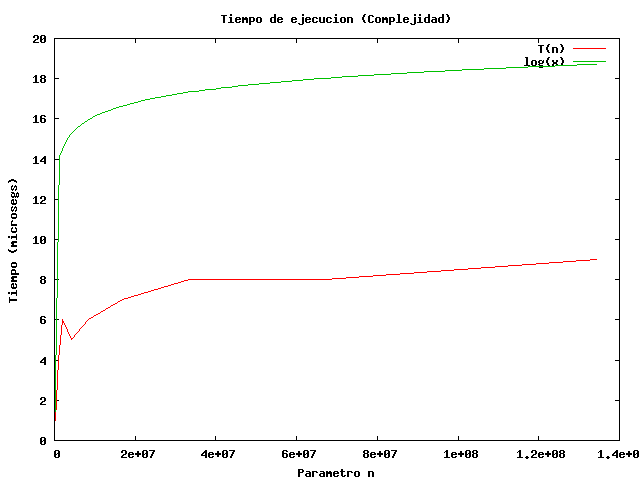
\includegraphics[width=0.7\textwidth]{Plots/Ej3-Complejidad.png}
% \begin{center}
% Figura 3.1
% \end{center}
% \end{center}

Como se puede observar en el gr\'afico, los tiempos de ejecuci\'on del algoritmo son muy bajos en relaci\'on al tama\~{n}o de la entrada. Esta fue la raz\'on por la que se descart\'o probar s\'olo casos peque\~{n}os para verificar la eficiencia del algoritmo y se opt\'o por analizar casos en el que el tama\~{n}o de la entrada creciera exponencialmente. A simple vista se puede observar que el gr\'afico de la funci\'on que mide el tiempo tiene el mismo comportamiento que la funci\'on de complejidad te\'orica. De este modo, adem\'as de la demostraci\'on te\'orica de la complejidad, se obtiene una prueba emp\'irica de que esta misma es correcta.

\section*{Conclusiones}

Este ejercicio nos hizo utilizar la t\'cnica de Divide and Conquer y nos mostr\'o varias de sus caracter\'isticas. La necesidad de utilizar 
esta t\'ecnica result\'o de la b\'usqueda de disminuir la complejidad lineal propuesta por la solución trivial.
	La complejidad obtenida muestra la relaci\'on que hay en ciertos algoritmos Divide and Conquer, entre el costo temporal de resolverlo 
y la cantidad de elementos de entrada. En este caso ni siquiera fue necesario leer cada uno de los elementos gracias a que cont\'abamos con
el orden de los vectores.
	En nuestro algoritmo el costo de cada una de las divisiones y cada una de las conquistas es contante, permitiendo que s\'olo 
la cantidad de llamadas a problemas m\'as peque\~{n}os defina la complejidad. Esta propiedad no logra s\'olo ser eficiente, sino que adem\'as, 
permite un c\'alculo sencillo de la complejidad temporal. En las pruebas emp\'iricas realizadas, puede observarse como el tiempo que toma realizar nuestro algoritmo,
es notablemente inferior al del tama\~{n}o de la entrada. Cabe destacar que nuestro algoritmo hace una cantidad similar de operaciones en todos los casos (para un mismo
tama\~{n}o de la entrada), ya que para calcular la mediana siempre debe llegar al caso base. Esto ayuda a la demostraci\'on de la correctitud del algortimo y lo hace 
m\'as natural. Puede observarse en el gr\'afico de nuestras pruebas, la ausencia de grandes picos, que muestra emp\'iricamente que para entradas de similar tama\~{n}o, el 
tiempo demandado ser\'a similar .
	Realizar este ejercicio tambi\'en nos mostr\'o la sencillez y la naturalidad con la que se pueden implementar los algoritmos divide and conquer mediante un 
m\'etodo recursivo, aunque claro, esto puede cambiar dependiendo de lo complejo que sea implementar la divisi\'on y la conquista. 
	En definitiva, se puede concluir que en ciertos casos,y en este en particular, los algoritmos Divide and Conquer son f\'aciles de implementar, eficientes en el peor caso, y es 
sencillo calcular su complejidad.


\end{document}